\documentclass{beamer}
\usepackage[utf8]{inputenc}

\usetheme{Madrid}
\usecolortheme{default}
\usepackage{amsmath,amssymb,amsfonts,amsthm}
\usepackage{txfonts}
\usepackage{tkz-euclide}
\usepackage{listings}
\usepackage{adjustbox}
\usepackage{array}
\usepackage{tabularx}
\usepackage{gvv}
\usepackage{lmodern}
\usepackage{circuitikz}
\usepackage{tikz}
\usepackage{graphicx}

\setbeamertemplate{page number in head/foot}[totalframenumber]

\usepackage{tcolorbox}
\tcbuselibrary{minted,breakable,xparse,skins}



\definecolor{bg}{gray}{0.95}
\DeclareTCBListing{mintedbox}{O{}m!O{}}{%
  breakable=true,
  listing engine=minted,
  listing only,
  minted language=#2,
  minted style=default,
  minted options={%
    linenos,
    gobble=0,
    breaklines=true,
    breakafter=,,
    fontsize=\small,
    numbersep=8pt,
    #1},
  boxsep=0pt,
  left skip=0pt,
  right skip=0pt,
  left=25pt,
  right=0pt,
  top=3pt,
  bottom=3pt,
  arc=5pt,
  leftrule=0pt,
  rightrule=0pt,
  bottomrule=2pt,

  colback=bg,
  colframe=orange!70,
  enhanced,
  overlay={%
    \begin{tcbclipinterior}
    \fill[orange!20!white] (frame.south west) rectangle ([xshift=20pt]frame.north west);
    \end{tcbclipinterior}},
  #3,
}
\lstset{
    language=C,
    basicstyle=\ttfamily\small,
    keywordstyle=\color{blue},
    stringstyle=\color{orange},
    commentstyle=\color{green!60!black},
    numbers=left,
    numberstyle=\tiny\color{gray},
    breaklines=true,
    showstringspaces=false,
}
%------------------------------------------------------------
%This block of code defines the information to appear in the
%Title page
\title %optional
{2.2.24}
\date{\today}
%\subtitle{A short story}

\author % (optional)
{Shivam Sawarkar \\ AI25BTECH11031}



\begin{document}


\frame{\titlepage}
\begin{frame}{Question (2.2.24)}
    If $\hat{i}+\hat{j}+\hat{k}$,$2\hat{i}+5\hat{j}$,$3\hat{i}+2\hat{j}-3\hat{k}$ and $\hat{i}-6\hat{j}-\hat{k}$ are the position vectors of the point $\Vec{A}$,$\Vec{B}$,$\Vec{C}$ and $\Vec{D}$ respectively, then find the angle between $\Vec{AB}$ and $\Vec{CD}$. Deduce that $\Vec{AB}$ and $\Vec{CD}$ are collinear.
\end{frame}

\begin{frame}{Solution}
    Given points are
\begin{align}
\vec{A}=\myvec{1\\1\\1}, \quad
\vec{B}=\myvec{2\\5\\0}, \quad
\vec{C}=\myvec{3\\2\\-3}, \quad
\vec{D}=\myvec{1\\-6\\-1}.
\end{align}

\begin{align}
\vec{AB} = \vec{B}-\vec{A} = \myvec{1\\4\\-1}, 
\qquad
\vec{CD} = \vec{D}-\vec{C} = \myvec{-2\\-8\\2}.
\end{align}
\end{frame}

\begin{frame}{Solution}
    The angle $\theta$ between $\vec{AB}$ and $\vec{CD}$ is given by
\begin{align}
\cos\theta = \frac{\vec{AB}^{\top}\vec{CD}}{\norm{AB}\norm{CD}}.
\end{align}

\begin{align}
\vec{AB}^T \vec{CD} =
\myvec{1 & 4 & -1}
\myvec{-2\\-8\\2}
= (1)(-2)+(4)(-8)+(-1)(2) = -36.
\end{align}

\begin{align}
\norm{AB} =3\sqrt{2}, 
\qquad
\norm{CD} = 6\sqrt{2}.
\end{align}
\end{frame}

\begin{frame}{Solution}
    \begin{align}
\cos\theta = \frac{-36}{(3\sqrt{2})(6\sqrt{2})} 
= \frac{-36}{36}=-1.
\end{align}

Hence,
\begin{align}
\theta = \cos^{-1}(-1) = \pi \;\;(180^\circ).
\end{align}

Since, angle between vectors is $180^\circ$ the given vectors are collinear
\end{frame}

\begin{frame}{Solution}
    Proof of collinearity by rank method \\
Let, 
\begin{align}
    \vec{P}=\myvec{B-A & D-C} \\ 
    \vec{P}=\myvec{1 & -2 \\ 
                   4 & -8 \\
                   -1 & 2} \\ 
    \vec{P}^T=\myvec{1 & 4 & -1 \\
                     -2 & -8 & 2} \\ 
    R_2 \rightarrow R_2 - 2R_1 \\ 
    \vec{P}^T = \myvec{1 & 4 & -1 \\ 
                       0 & 0 & 0} \\ 
    rank\vec{P}=rank\vec{P}^T = 1 \\ 
\end{align}

Thus the given vectors are collinear.
\end{frame}

\begin{frame}{Plot}
    \begin{figure}
        \centering
        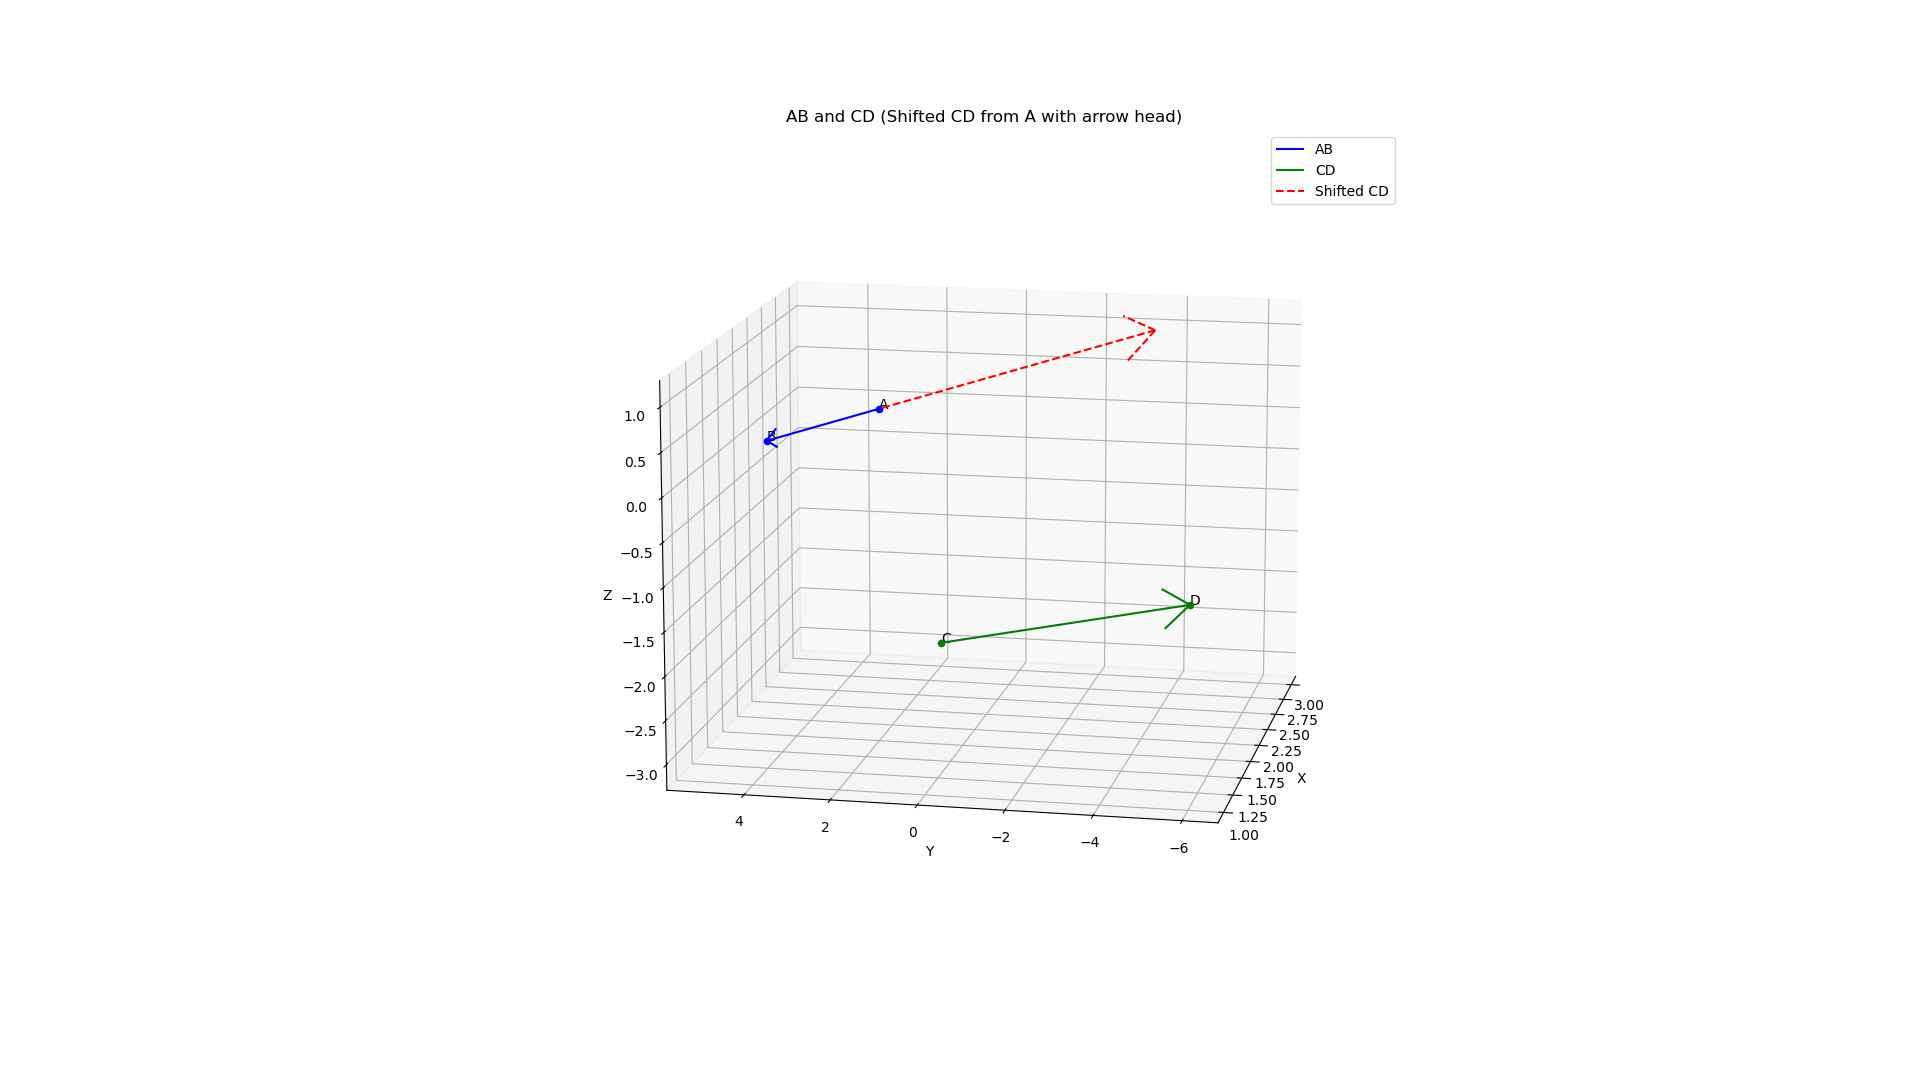
\includegraphics[width=1\linewidth]{Figs/plot3_1.png}
        \caption{}
        \label{fig:placeholder}
    \end{figure}
\end{frame}

\begin{frame}[fragile]{C Code}
    \begin{verbatim}
    #include <stdio.h>
    #include <math.h>

    // Function to compute dot product of two vectors
    double dot_product(double v1[3], double v2[3]) {
        return v1[0]*v2[0] + v1[1]*v2[1] + v1[2]*v2[2];
    }

    // Function to compute norm of a vector
    double norm(double v[3]) {
        return sqrt(v[0]*v[0] + v[1]*v[1] + v[2]*v[2]);
    }
    \end{verbatim}
\end{frame}

\begin{frame}[fragile]{C Code}
    \begin{verbatim}
    int main() {
        double A[3], B[3], C[3], D[3];
        double AB[3], CD[3];
        int i;
        // Input points
        printf("Enter coordinates of A (x y z): ");
        scanf("%lf %lf %lf", &A[0], &A[1], &A[2]);
    
        printf("Enter coordinates of B (x y z): ");
        scanf("%lf %lf %lf", &B[0], &B[1], &B[2]);
    
        printf("Enter coordinates of C (x y z): ");
        scanf("%lf %lf %lf", &C[0], &C[1], &C[2]);
    
        printf("Enter coordinates of D (x y z): ");
        scanf("%lf %lf %lf", &D[0], &D[1], &D[2]);
    \end{verbatim}
\end{frame}

\begin{frame}[fragile]{C Code}
    \begin{verbatim}
        // Compute vectors AB and CD
        for (i = 0; i < 3; i++) {
            AB[i] = B[i] - A[i];
            CD[i] = D[i] - C[i];
        }
    
        // Print vectors
        printf("\nVector AB = (%.2lf, %.2lf, %.2lf)\n", AB[0], AB[1], AB[2]);
        printf("Vector CD = (%.2lf, %.2lf, %.2lf)\n", CD[0], CD[1], CD[2]);
    
        // Compute angle
        double dot = dot_product(AB, CD);
        double cos_theta = dot / (norm(AB) * norm(CD));
        int x = (cos_theta * 100);
        double y = x/100;
        double theta = acos(y)*180/M_PI;
    \end{verbatim}
\end{frame}

\begin{frame}[fragile]{C Code}
    \begin{verbatim}
        printf("\nDot product = %.2lf\n", dot);
        printf("cos(theta) = %.2lf\n", cos_theta);
        printf("Angle between AB and CD = %.2lf degrees\n", theta);
    
        if (cos_theta == 1 || -1){
            printf("\n AB and CD are collinear.\n");
        } else {
            printf("\n AB and CD are not collinear.\n");
        }
    
        return 0;
    }
    \end{verbatim}
\end{frame}

\begin{frame}[fragile]{Python Code}
    \begin{verbatim}
    import numpy as np
    
    # Function to read a point from user
    def read_point(name):
        coords = input(f"Enter coordinates of {name} (x y z): ").split()
        return np.array(list(map(float, coords)))
    
    # Input points
    A = read_point("A")
    B = read_point("B")
    C = read_point("C")
    D = read_point("D")
    
    # Vectors
    AB = B - A
    CD = D - C
    \end{verbatim}
\end{frame}

\begin{frame}[fragile]{Python Code}
    \begin{verbatim}
    # Step 1: Angle between AB and CD
    dot_product = np.dot(AB, CD)
    norms = np.linalg.norm(AB) * np.linalg.norm(CD)
    cos_theta = dot_product / norms
    x = cos_theta*100
    y = int(x)/100
    theta_deg = np.degrees(np.arccos(y))
    
    # Step 2: Rank method for collinearity
    M = np.column_stack((AB, CD))   # Matrix with AB and CD as columns
    rank = np.linalg.matrix_rank(M)
    \end{verbatim}
\end{frame}

\begin{frame}[fragile]{Python Code}
    \begin{verbatim}
    # Print results
    print("\n--- Results ---")
    print("Vector AB:", AB)
    print("Vector CD:", CD)
    print("Dot product =", dot_product)
    print("cos(theta) =", y)
    print("Angle between AB and CD =", theta_deg, "degrees")
    print("Matrix M:\n", M)
    print("Rank of M =", rank)
    
    if rank == 1:
        print("Vectors AB and CD are collinear.")
    else:
        print("Vectors AB and CD are not collinear.")
    \end{verbatim}
\end{frame}


\end{document}